%--------------------------------------------------------------------------
% !TEX root = 5Blman.tex
% induction.tex
% 2013.01.07 changed to 2col format
%--------------------------------------------------------------------------
\chapter{Electromagnetic Induction}

\begin{multicols}{2}
%---------------------------------------------------------------------
\section{Purpose}
The purpose of this laboratory exercise is to explore the phenomenon of electromagnetic induction.  Electromagnetic induction is the creation of an emf using magnetic fields.  It is the basis of most electric generators as well as being responsible for a number of other effects.  The connections between electric and magnetic forces shown by electromagnetic induction is also evidence of the underlying unity of physical laws.

%---------------------------------------------------------------------
\section{Preparation}
Reread the sections in your text on electromagnetic induction before coming to lab. Pay special attention to the concepts of magnetic flux, Faraday's law of induction, and Lenz's law.  You should also review the \textsf{right hand rule for forces} of magnetic fields produced by currents --- in wires and by loops of wire.  You should be able to apply the \textsf{right hand rule for forces} to similar situations as shown in \reffig{f:fig11} to perform this lab.


%\begin{figure}[hbt]
%	\centering
%	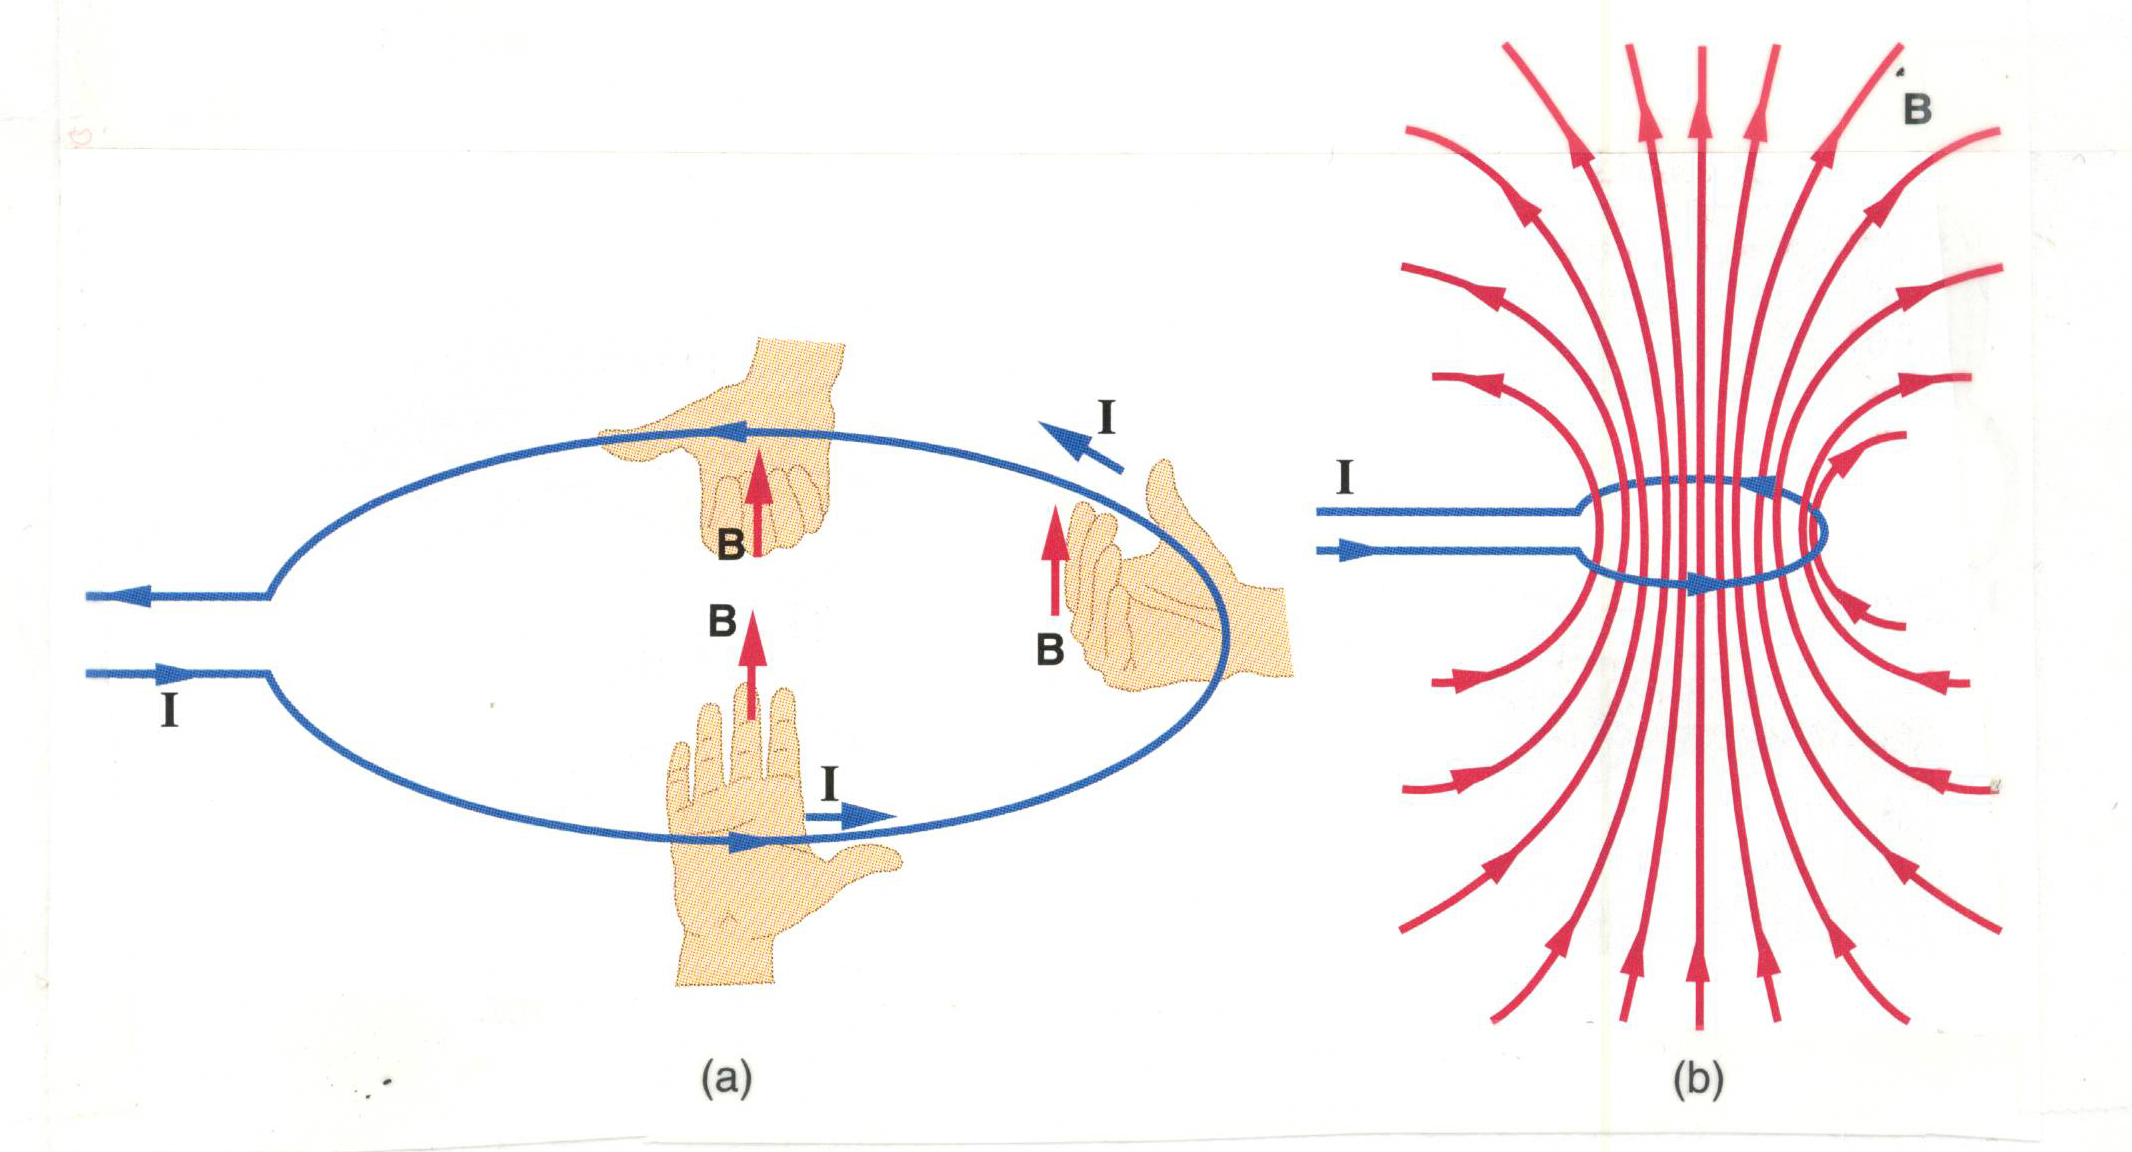
\includegraphics[scale=0.6]{5bgraf/fig_11}
%	\caption{Right hand rule for magnetic fields}
%	\label{f:fig11}
%\end{figure}

\begin{center}
	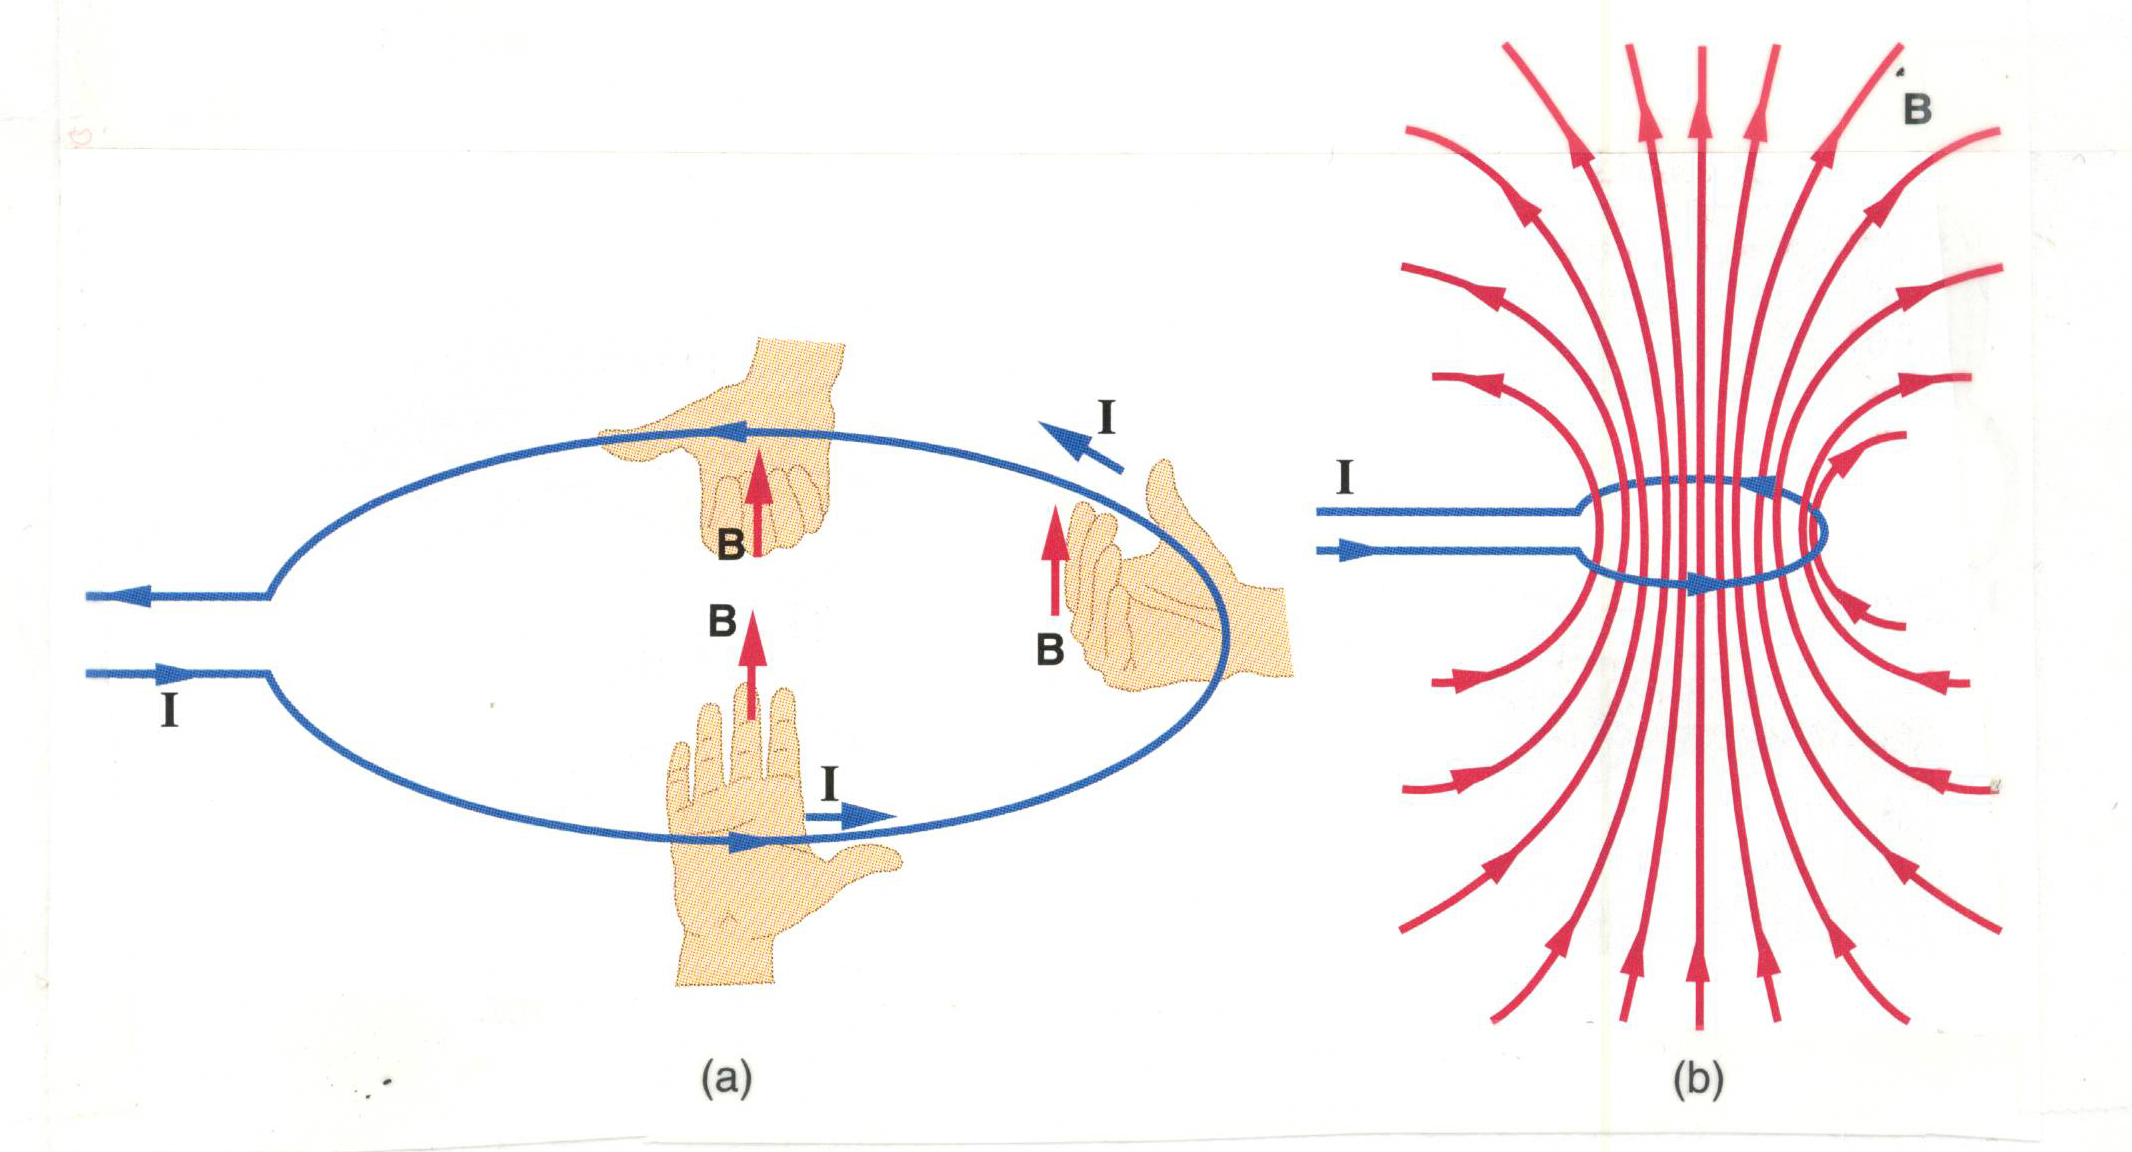
\includegraphics[scale=0.6]{5bgraf/fig_11}
	\mfcaption{Right hand rule for magnetic fields}
	\label{f:fig11}
\end{center}

\paragraph{Short problem}
Suppose the current in coil 1 is increasing in \reffig{f:fig12}.  Explain the direction of the current induced in coil 2 using Faraday's law, Lenz's law, and RHR-2.  You may be asked to turn in your explanation at the beginning of class as a short preparatory quiz.

%\begin{figure}
%	\centering
%	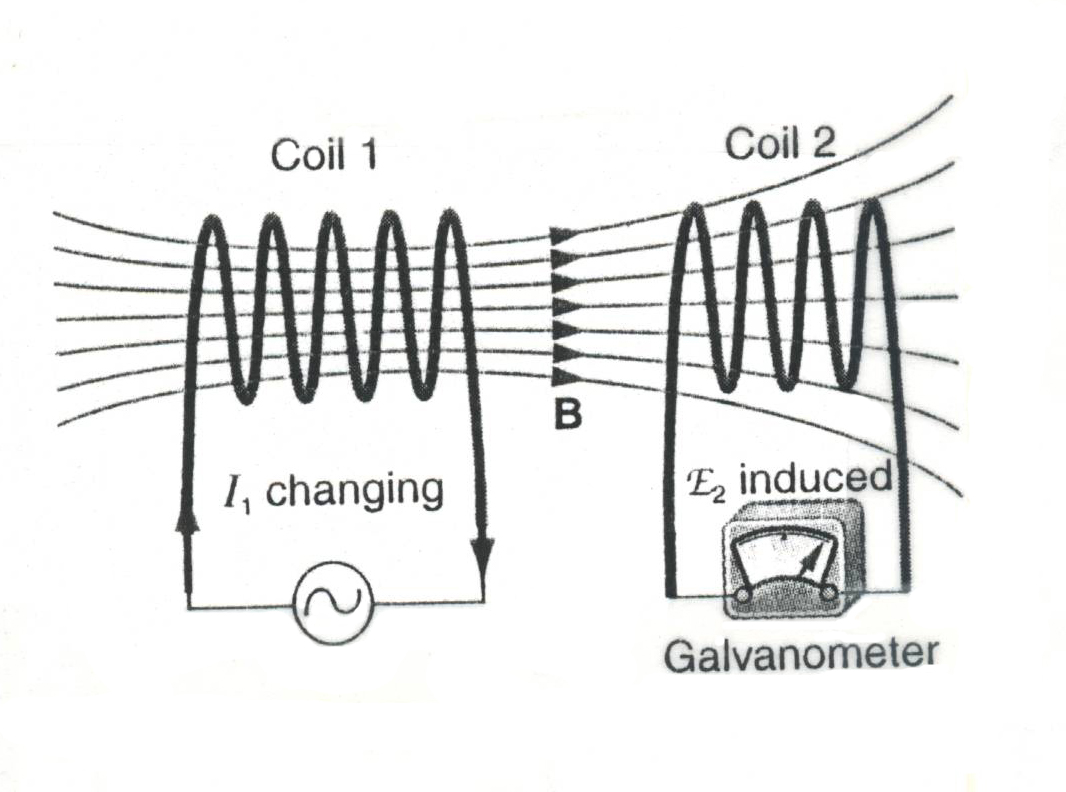
\includegraphics[scale=0.8]{5bgraf/fig_12}
%	\caption{A changing current in one coil induces an EMF in another coil}
%	\label{f:fig12}
%\end{figure}

\begin{center}
	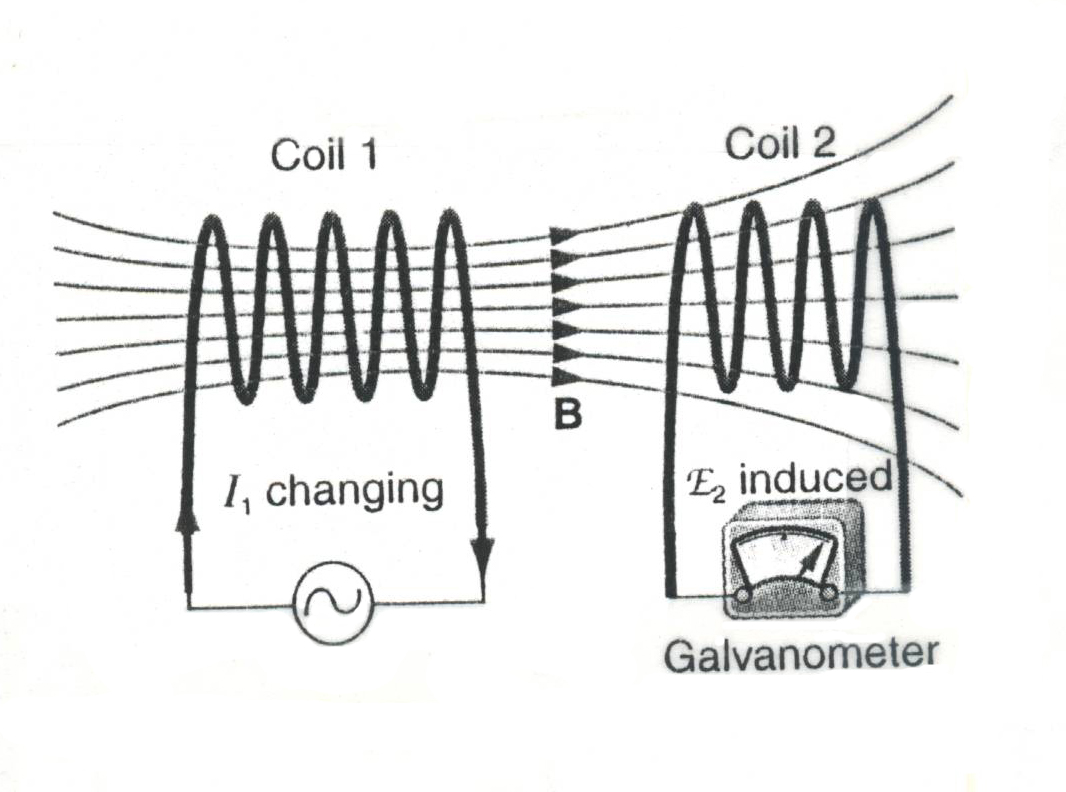
\includegraphics[scale=0.8]{5bgraf/fig_12}
	\mfcaption{A changing current in one coil induces an EMF in another coil}
	\label{f:fig12}
\end{center}

%---------------------------------------------------------------------
\section{Experimental Set-Up}
You will use two coils in a series of activities.  These are shown in \reffig{f:fig13} as one of the configurations you will explore.  The primary coil is the one that you connect to a battery and switch.  The secondary coil is the one you connect to a galvanometer.  Current into the + side of the galvanometer causes a deflection of the meter to the right: this allows you to determine the direction and relative magnitude of any current induced in the secondary.


%\begin{figure}
%	\centering
%	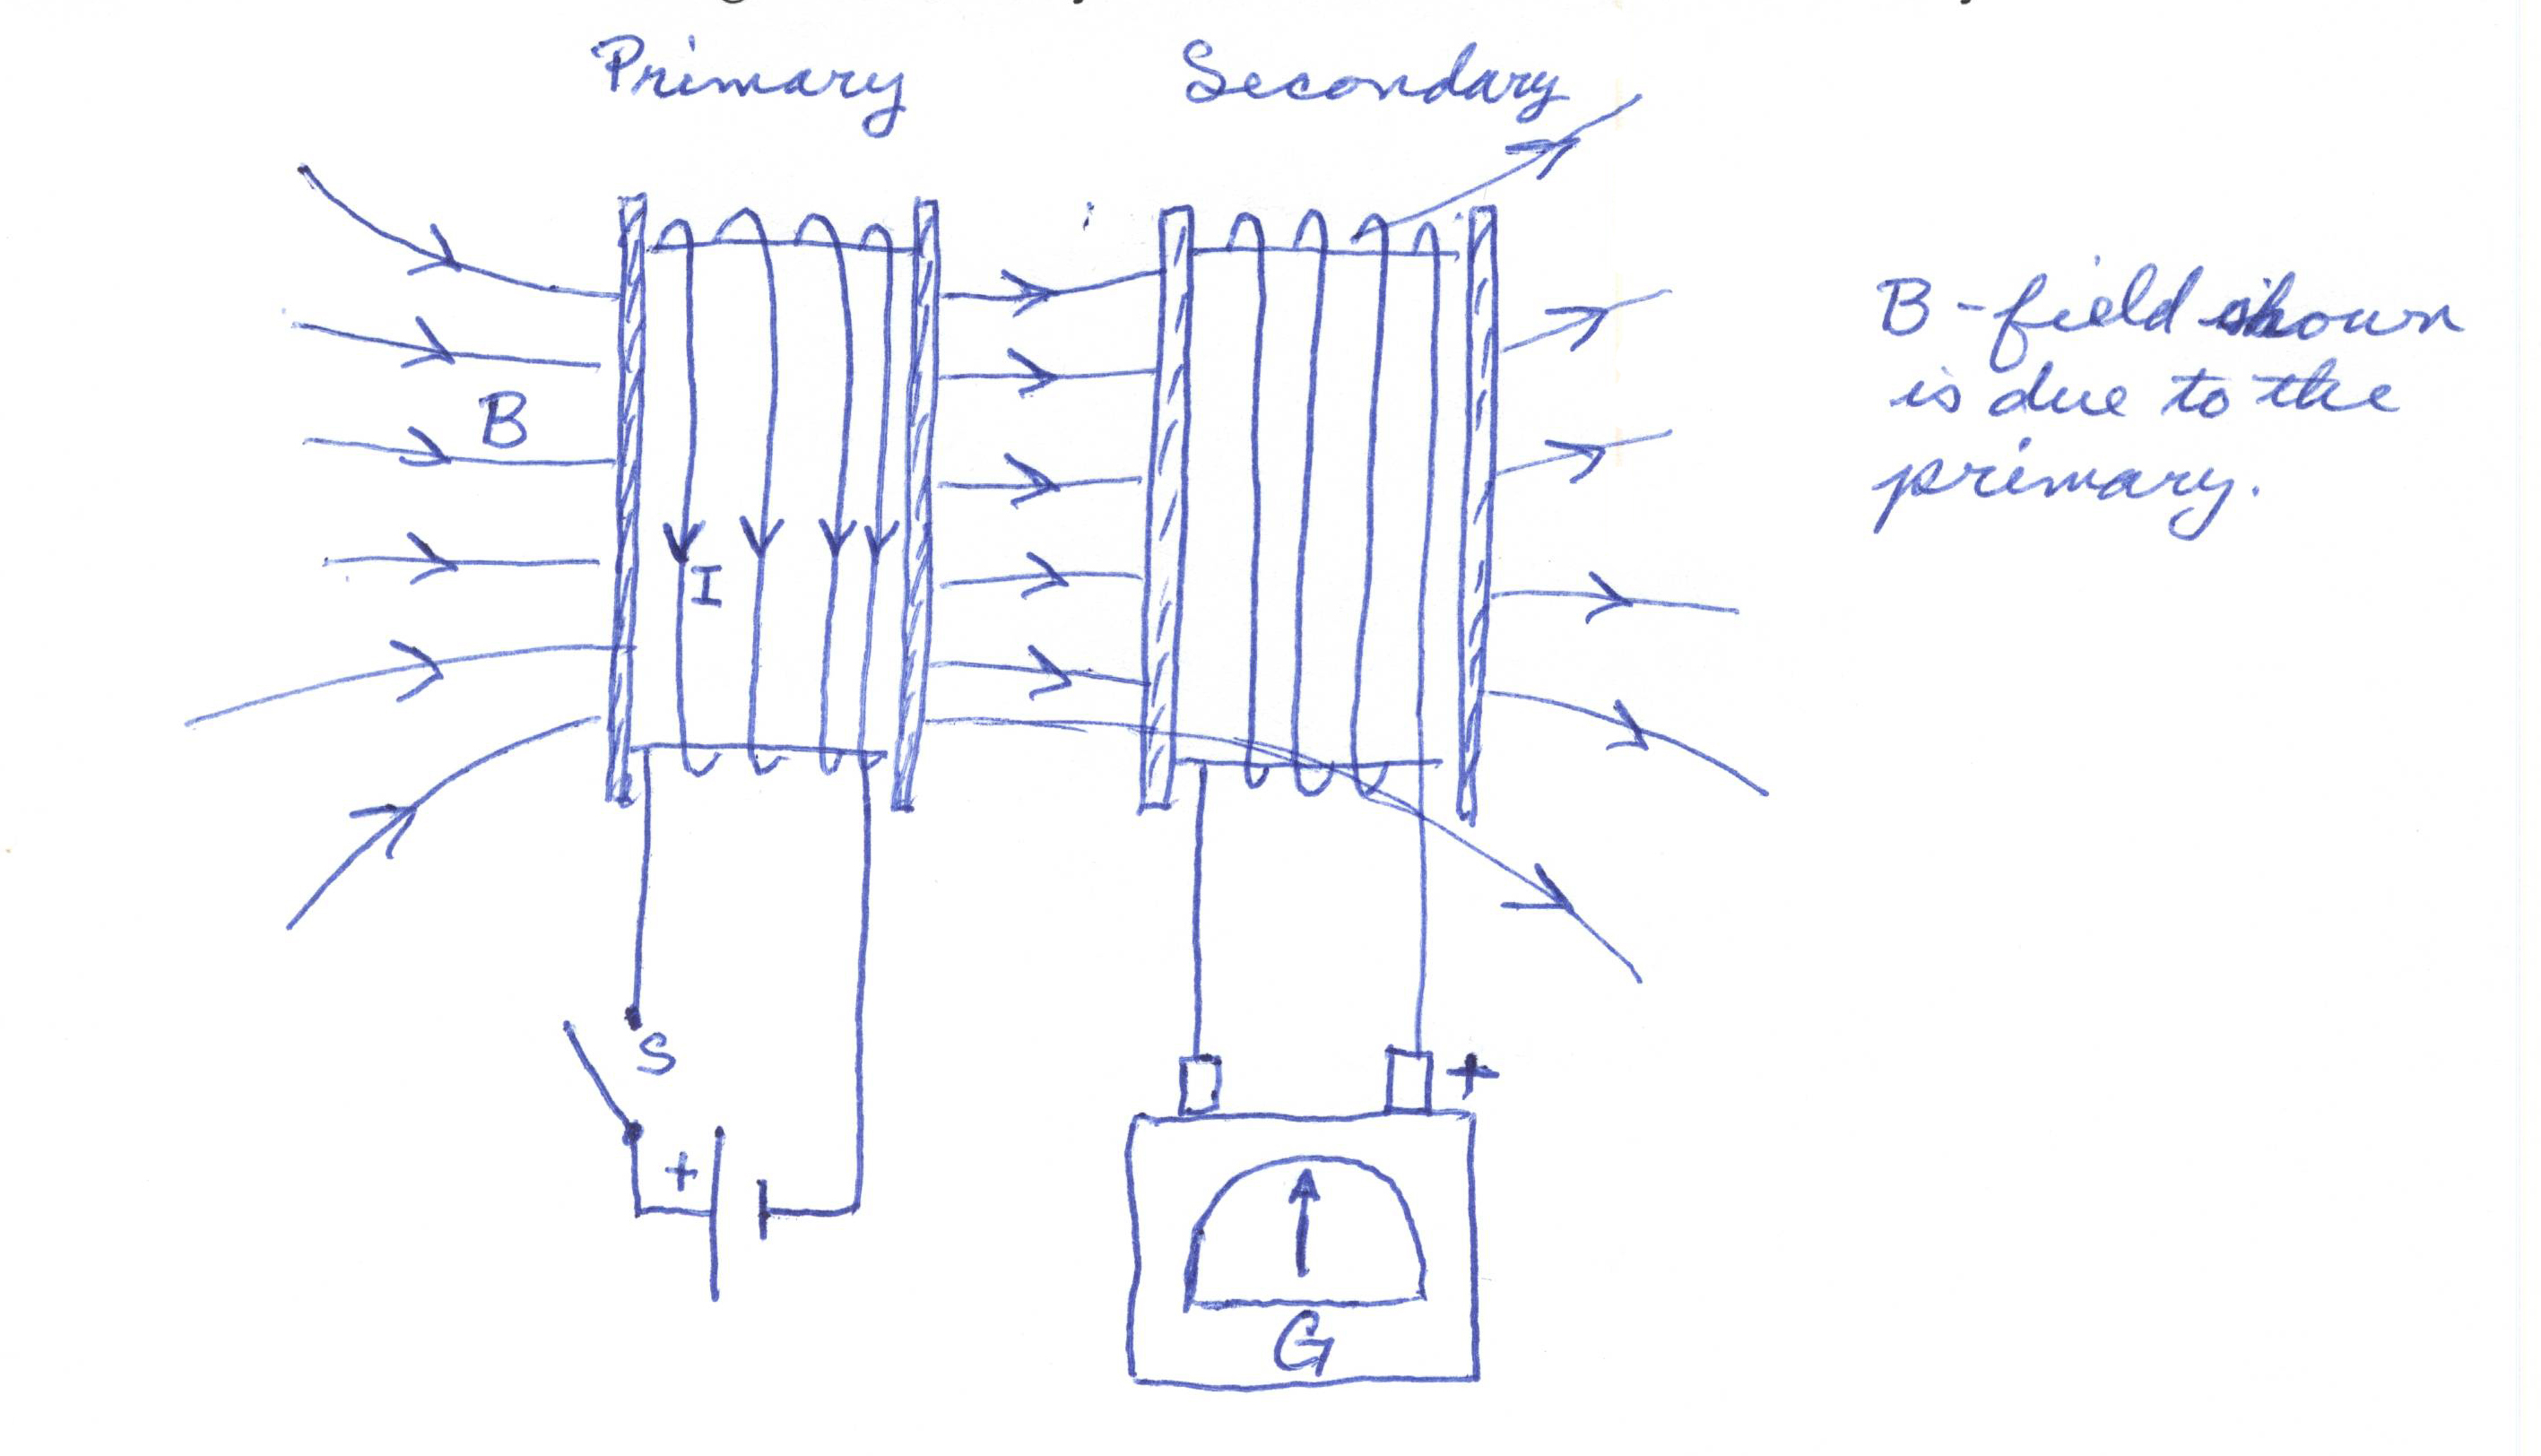
\includegraphics[scale=0.6]{5bgraf/fig_13}
%	\caption{Primary and secondary coils illustrate Lenz's law}
%	\label{f:fig13}
%\end{figure}

\begin{center}
	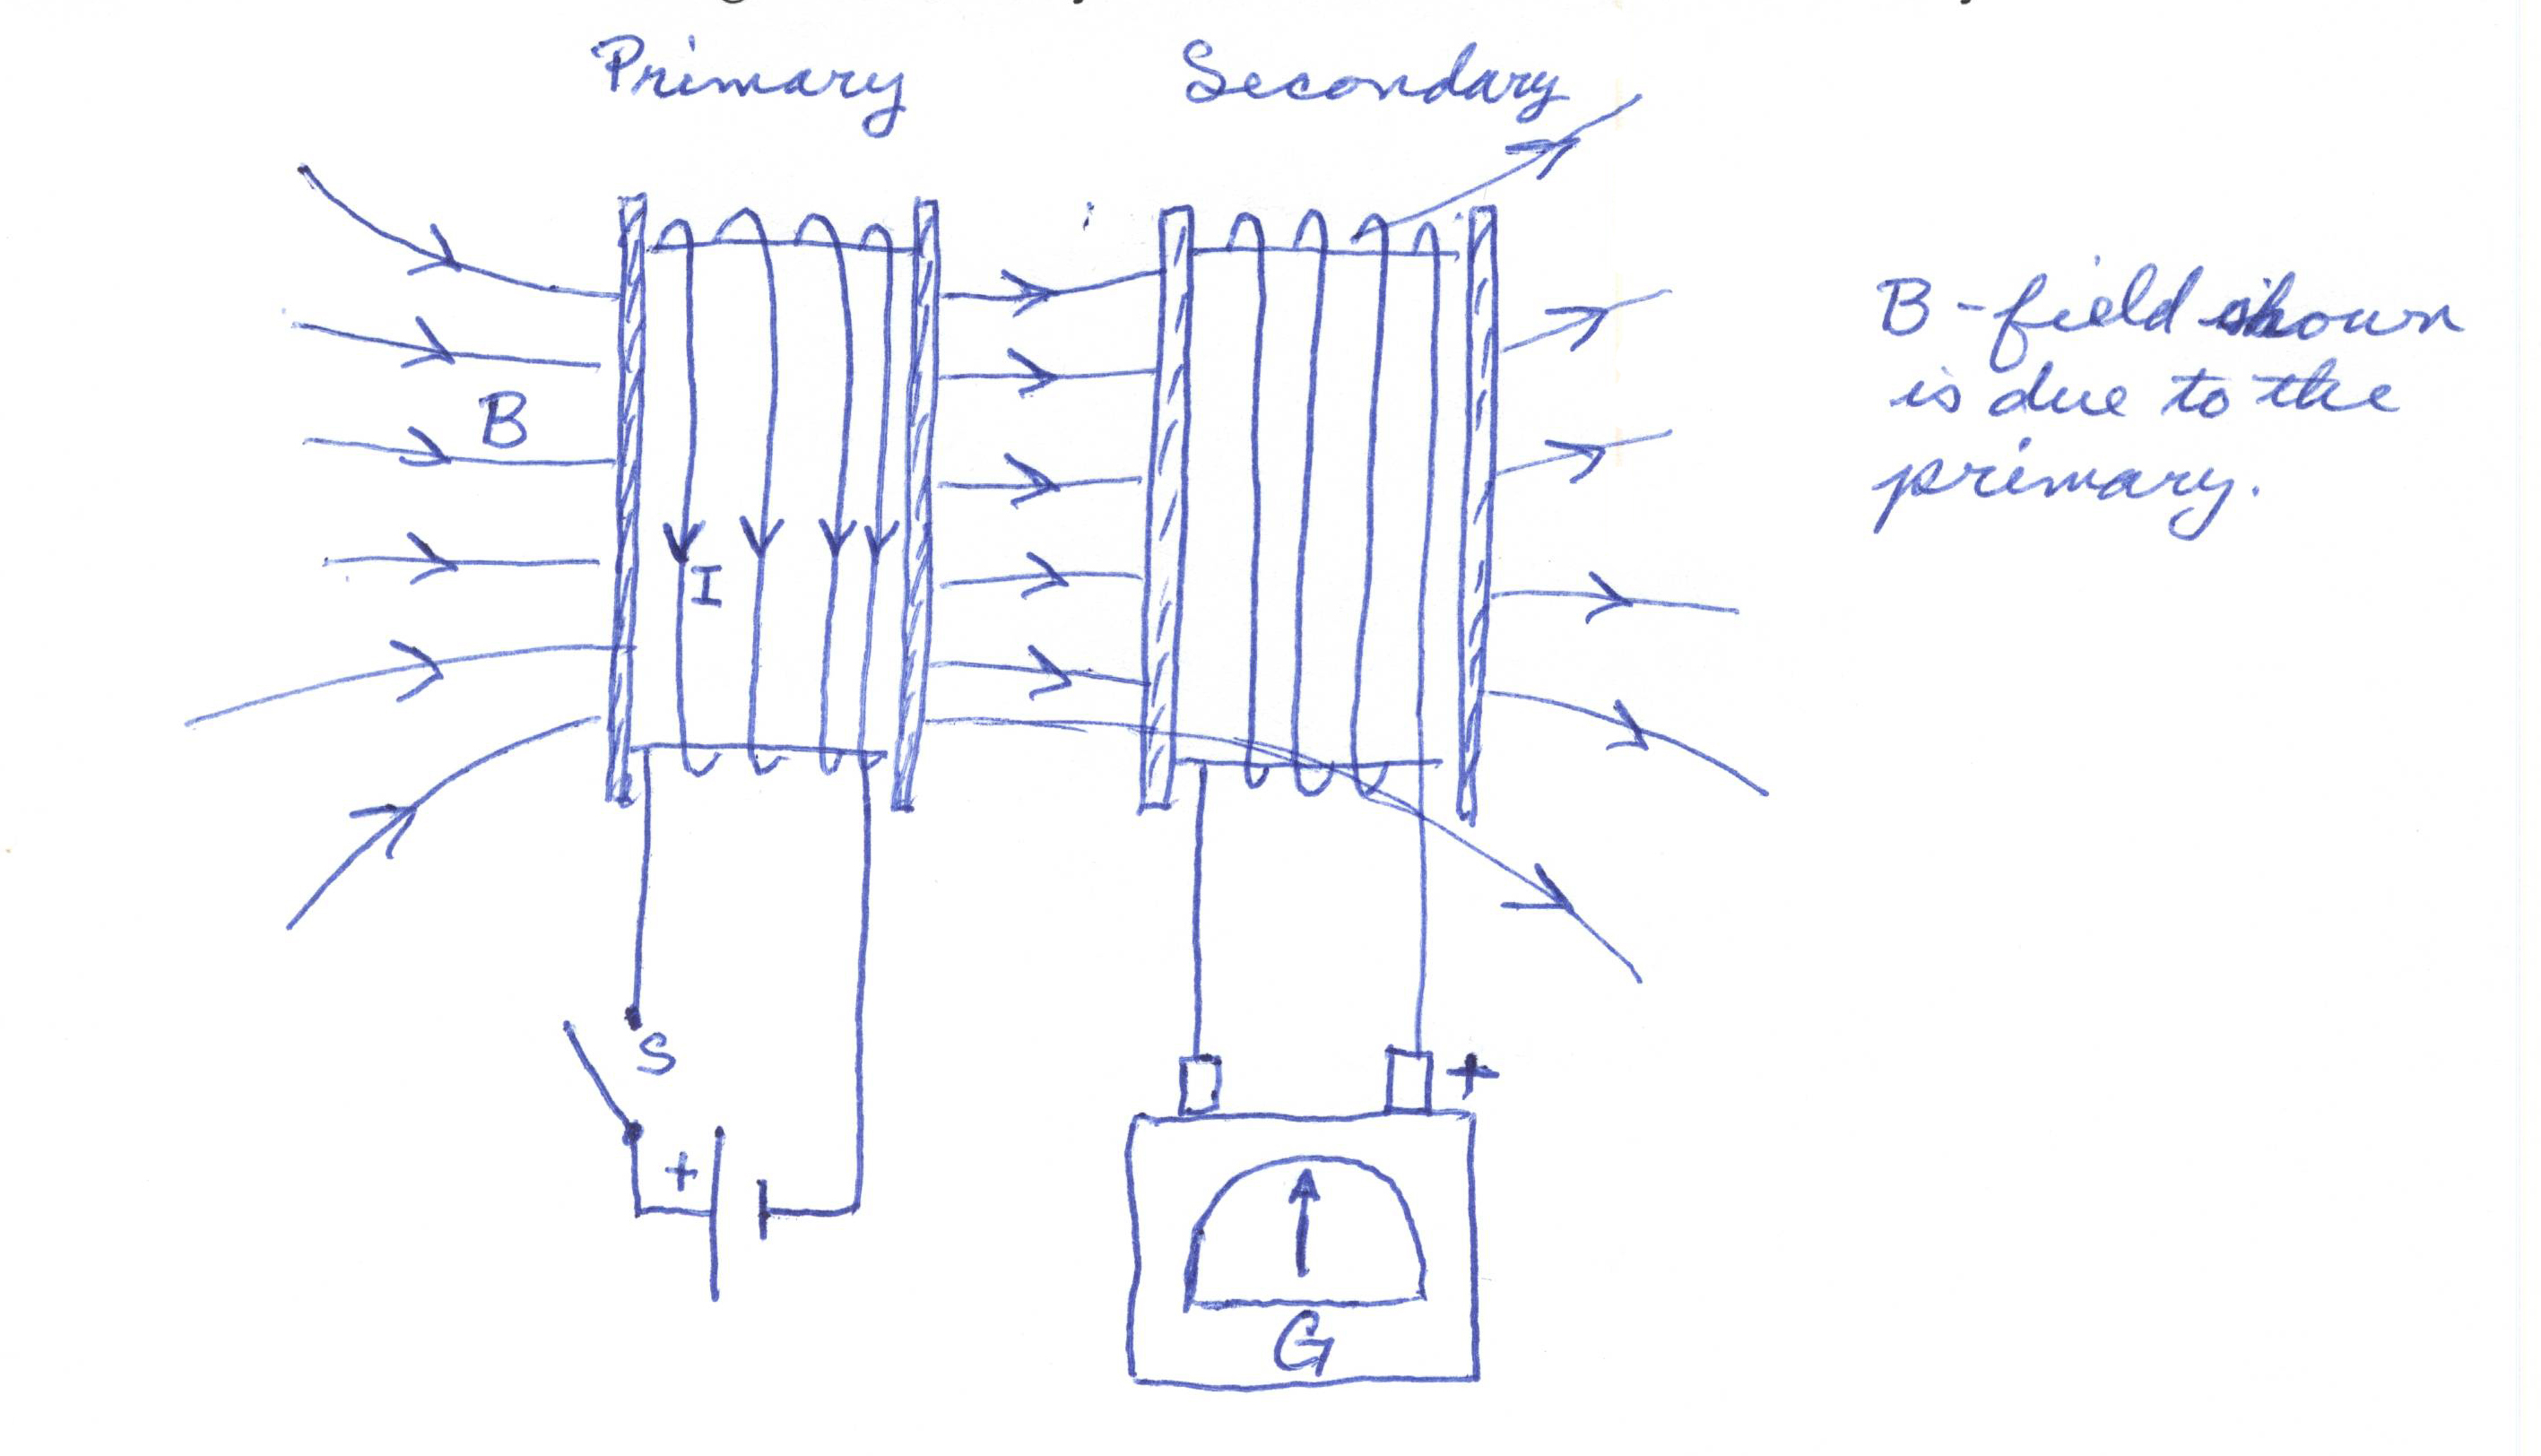
\includegraphics[scale=0.6]{5bgraf/fig_13}
	\mfcaption{Primary and secondary coils illustrate Lenz's law}
	\label{f:fig13}
\end{center}

%---------------------------------------------------------------------
\section{Exploring Magnetic Induction}

\subsection{Activity: Magnetic field and current direction}
% Verification of RHR-2
\begin{enumerate}
	 \item 	Use the primary coil and the small compasses to verify the \textsf{right hand rule for forces} -- that is, verify the relationship of the direction of the magnetic field to the direction of current through the primary coil.
	 \item 	Note that current flows out of the + terminal of the battery and that the magnetic field direction is (by definition) the direction that the north seeking end of a compass points.  You should explore the direction of the field inside and outside of the coil first for current flowing in one direction and again for current flowing in the opposite direction.
	 \item 	Make drawings that indicate the direction of current and magnetic field in both cases.  Explain how the direction of the field is consistent with the \textsf{right hand rule for forces}.
\end{enumerate}

\subsection{Activity: Induced emf by a coil} \label{s:coilind}
% Emf $E$ induced in the secondary coil by the primary coil
	Line up the primary and secondary coils in an arrangement similar to that in \reffig{f:fig13} above with the primary connected to the battery and switch and the secondary connected to the galvanometer.  Be certain that the windings of both coils are in the same direction: that is, both clockwise or both counterclockwise. 
	
	Explain all observations by making drawings and using Faraday's law, Lenz's law, and the \textsf{right hand rule for forces}
\begin{enumerate}
	 \item Open and close the switch.  What direction does the galvanometer deflect?  Does it show a deflection at all times?  
	\item Close the switch and leave it closed.  Move the secondary away from the primary and bring it back.  Note the reaction of the galvanometer and any dependence on how fast the secondary is moved.
	\item Repeat part ($1$), but move the primary instead of the secondary cois.
	\item Use an iron rod to link the primary and secondary coils instead of the wood rod.  Starting with the coils separated by 10 cm, open and close the switch to the primary.  Record the relative magnitude of the deflection of the galvanometer then decrease the separation of the coils to 9 cm, then 8 cm, and so on.  Make a graph of the galvanometer deflection versus distance between the coils. 
\end{enumerate}

\subsection{Activity: Induced emf by a magnet}
% Emf $E$ induced in the secondary coil by a bar magnet
\begin{enumerate}
	 \item First verify with small compasses that the bar magnet has its poles correctly labeled.
	\item  Remove the primary coil and keep the secondary coil connected to the galvanometer.  Thrust the north pole of the bar magnet into the core of the secondary coil.  Then pull it out.  Repeat with the south pole of the bar magnet.  Examine the effect of the speed of the motion.  
	\item Explain all observations by making drawings and using Faraday's law, Lenz's law, and the \textsf{right hand rule for forces}.  Also verify that the observations are consistent with those obtained in activity \ref{s:coilind}. 
\end{enumerate}

%---------------------------------------------------------------------
\section{Conclusions}
 What aspects of Faraday's law, Lenz's law, and the \textsf{right hand rule for forces} have you verified in today's laboratory exercise?
 
% \clearpage
%\newpage
%\includegraphics*[width=\textwidth,trim=120 80 80 120,clip]{5bgraf/pslabgrid} 

\end{multicols}
%--------------------------------------------------------------------------
\endinput
%--------------------------------------------------------------------------
